

%% AAPT Physics Bowl Exams Questions
%%----------------------------------------


%% This section has XX problems


%% PhysicsBowl 2015
%%----------------------------------------
\element{aapt}{ %% Bowl-C2
\begin{question}{bowl-2015-q44}
    Which one of the following choices is most associated with the following statement:
        ``When the pressure of a gas is held constant,
        the volume of the gas is directly proportional to the temperature.''?
    \begin{multicols}{2}
    \begin{choices}
        \wrongchoice{Newton's Law}
        \wrongchoice{Boyle's Law}
        \wrongchoice{Avogadro's Law}
        \wrongchoice{Graham's Law}
      \correctchoice{Charles's Law}
    \end{choices}
    \end{multicols}
\end{question}
}


%% PhysicsBowl 2014
%%----------------------------------------
\element{aapt-C2}{ %% Bowl-C2
\begin{question}{bowl-2014-q37}
    A new element is discovered and named PhysicsBowlium (atomic symbol \emph{Phys}).
    Its entry onto the standard periodic table of elements appears as in the figure
        (with Helium shown as well).
    \begin{center}
    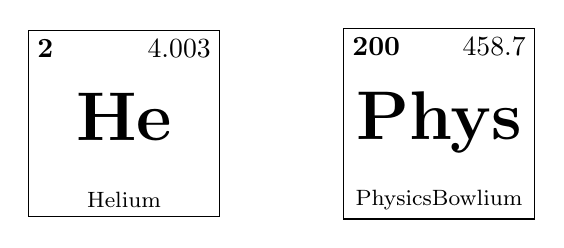
\begin{tikzpicture}
        \node[draw,rectangle,anchor=center] at (-2,0) {
            \begin{minipage}{2.2cm}
                \centering
                {\textbf{2} \hfill 4.003}
                \linebreak \linebreak
                {\Huge\textbf{He}}
                \linebreak \linebreak
                {{\footnotesize Helium}}
            \end{minipage}
        };
        \node[draw,rectangle,anchor=center] at (+2,0) {
            \begin{minipage}{2.2cm}
                \centering
                {\textbf{200} \hfill 458.7}
                \linebreak \linebreak
                {\Huge\textbf{Phys}}
                \linebreak \linebreak
                {{\footnotesize PhysicsBowlium}}
            \end{minipage}
        };
    \end{tikzpicture}
    \end{center}
    Given a sample of \emph{Phys} which acts as a perfect monatomic ideal gas,
        what is the root-mean-square speed of the atoms of the gas if
        the sample is at \SI{20}{\degreeCelsius}?
    \begin{multicols}{3}
    \begin{choices}
        \wrongchoice{\SI{1.04}{\meter\per\second}}
        \wrongchoice{\SI{4.00}{\meter\per\second}}
        \wrongchoice{\SI{33.0}{\meter\per\second}}
      \correctchoice{\SI{126}{\meter\per\second}}
        \wrongchoice{\SI{191}{\meter\per\second}}
    \end{choices}
    \end{multicols}
\end{question}
}


%% PhysicsBowl 2013
%%----------------------------------------
\element{aapt}{ %% Bowl-C2
\begin{question}{bowl-2013-q20}
    A sample of ideal gas at a temperature of \SI{40.0}{\degreeCelsius} is in a container of volume \SI{3.50e-2}{\meter\cubed}.
    If the pressure of the gas is \SI{0.50}{\atm},
        how many molecules of the gas are in the container?
    \begin{multicols}{2}
    \begin{choices}
        \wrongchoice{\num{4.05e18}}
        \wrongchoice{\num{4.10e20}}
        \wrongchoice{\num{4.05e21}}
      \correctchoice{\num{4.10e23}}
        \wrongchoice{\num{4.10e26}}
    \end{choices}
    \end{multicols}
\end{question}
}


%% PhysicsBowl 2012
%%----------------------------------------
\element{aapt}{ %% Bowl-C2
\begin{question}{bowl-2012-q40}
    Using the kinetic theory of gases, which one of the following choices best represents the RMS (root mean square) speed of \SI{58}{\gram} of monatomic ideal gas at a pressure of \SI{3.0}{\atm} in an enclosed container of volume \SI{6.0}{\liter}
    \begin{multicols}{3}
    \begin{choices}
        \wrongchoice{\SI{0.557}{\meter\per\second}}
        \wrongchoice{\SI{9.71}{\meter\per\second}}
        \wrongchoice{\SI{177}{\meter\per\second}}
      \correctchoice{\SI{307}{\meter\per\second}}
        \wrongchoice{\SI{3150}{\meter\per\second}}
    \end{choices}
    \end{multicols}
\end{question}
}


%% PhysicsBowl 2011
%%----------------------------------------
\element{aapt}{ %% Bowl-C2
\begin{question}{bowl-2011-q22}
    Three modes of an ideal gas occupy a container of volume \SI{2.5e-2}{\meter\cubed}.
    The pressure inside this container is \SI{5.00e5}{\pascal}.
    Which one of the following choices best represents the temperature of the gas?
    \begin{multicols}{3}
    \begin{choices}
        \wrongchoice{\SI{225}{\kelvin}}
      \correctchoice{\SI{500}{\kelvin}}
        \wrongchoice{\SI{775}{\kelvin}}
        \wrongchoice{\SI{1 500}{\kelvin}}
        \wrongchoice{\SI{50 800}{\kelvin}}
    \end{choices}
    \end{multicols}
\end{question}
}


%% PhysicsBowl 2010
%%----------------------------------------
\element{aapt}{ %% Bowl-C2
\begin{question}{bowl-2010-q20}
    A sample of ideal gas is in a container at a temperature of \SI{100}{\degreeCelsius} and a pressure of \SI{2.5}{\atm}.
    If the volume of the container is \SI{24}{\liter},
        approximately how many molecules of gas are in the container?
    \begin{multicols}{2}
    \begin{choices}
        \wrongchoice{\num{4.58e24}}
      \correctchoice{\num{1.23e24}}
        \wrongchoice{\num{6.25e23}}
        \wrongchoice{\num{4.53e22}}
        \wrongchoice{\num{1.21e22}}
    \end{choices}
    \end{multicols}
\end{question}
}


%% PhysicsBowl 2009
%%----------------------------------------
\element{aapt}{ %% Bowl-C2
\begin{question}{bowl-2009-q15}
    An ideal gas in a closed container of volume \SI{6.0}{\liter} is at a temperature of \SI{100}{\degreeCelsius}.
    If the pressure of the gas is \SI{2.5}{\atm},
        how many moles of gas are in the container?
    \begin{multicols}{3}
    \begin{choices}
      \correctchoice{\num{0.0048}}
        \wrongchoice{\num{0.018}}
        \wrongchoice{\num{0.49}}
        \wrongchoice{\num{1.83}}
        \wrongchoice{\num{490}}
    \end{choices}
    \end{multicols}
\end{question}
}


%% PhysicsBowl 2008
%%----------------------------------------
\element{aapt}{ %% Bowl-C2
\begin{question}{bowl-2008-q04}
    One mole of an ideal gas has a temperature of \SI{100}{\degreeCelsius}.
    If this gas fills the \SI{10.0}{\meter\cubed} volume of a closed container,
        what is the pressure of the gas?
    \begin{multicols}{2}
    \begin{choices}
        \wrongchoice{\SI{0.821}{\pascal}}
        \wrongchoice{\SI{3.06}{\pascal}}
        \wrongchoice{\SI{83.1}{\pascal}}
      \correctchoice{\SI{310}{\pascal}}
        \wrongchoice{\SI{1.84e24}{\pascal}}
    \end{choices}
    \end{multicols}
\end{question}
}

\element{aapt}{ %% Bowl-C2
\begin{question}{bowl-2008-q39}
    An ideal gas is enclosed in a container.
    The volume of the container is reduced to half the original volume at constant temperature.
    According to kinetic theory,
        what is the best explanation for the increase in pressure created by the gas?
    \begin{choices}
        \wrongchoice{The average speed of the gas particles decreases, but they hit the container wall more frequently.}
      \correctchoice{The average speed of the gas particles is unchanged, but they hit the container wall more frequently.}
        \wrongchoice{The average speed of the gas particles increases as does the frequency with which they hit the container walls.}
        \wrongchoice{The average speed of the gas particles increases, overcoming the decreases frequency that they hit the container walls.}
        \wrongchoice{The internal energy of the gas increases.}
    \end{choices}
\end{question}
}


%% PhysicsBowl 2006
%%----------------------------------------
\element{aapt}{ %% Bowl-C2
\begin{question}{bowl-2006-q25}
    A monoatomic ideal gas at pressure $P=\SI{e5}{\pascal}$ is in a container of volume $V=\SI{12}{\meter\squared}$ while at temperature $T=\SI{50}{\degreeCelsius}$.
    How many molecules of gas are in the container?
    \begin{multicols}{2}
    \begin{choices}
        \wrongchoice{\num{447}}
        \wrongchoice{\num{2888}}
        \wrongchoice{\num{6.02e23}}
      \correctchoice{\num{2.69e26}}
        \wrongchoice{\num{1.74e27}}
    \end{choices}
    \end{multicols}
\end{question}
}


%% PhysicsBowl 2005
%%----------------------------------------
\element{aapt}{ %% Bowl-C2
\begin{question}{bowl-2005-q40}
    A new monatomic ideal gas is discovered and named ``Physicsbowlium.''
    A pure \SI{4}{\mole} sample is sitting in a container at equilibrium in a \SI{20.0}{\degreeCelsius} environment.
    According to the kinetic theory of gases,
        what is the average kinetic energy per molecule for this gas?
    \begin{choices}
        \wrongchoice{\SI{4.14e-22}{\joule}}
        \wrongchoice{\SI{6.07e-21}{\joule}}
        \wrongchoice{\SI{2.02e-21}{\joule}}
        \wrongchoice{\SI{3652}{\joule}}
      \correctchoice{The molar mass of the gas is needed to answer this question.}
    \end{choices}
\end{question}
}


%% PhysicsBowl 1997
%%----------------------------------------
\element{aapt}{ %% Bowl-C2
\begin{question}{bowl-1997-q26}
    The average speed of the atoms of a gas at \SI{100}{\kelvin} is \SI{200}{\meter\per\second}.
    What would most nearly be the average speed of the atoms at \SI{300}{\kelvin}?
    \begin{multicols}{2}
    \begin{choices}
        \wrongchoice{\SI{67}{\meter\per\second}}
        \wrongchoice{\SI{140}{\meter\per\second}}
        \wrongchoice{\SI{200}{\meter\per\second}}
      \correctchoice{\SI{350}{\meter\per\second}}
        \wrongchoice{\SI{600}{\meter\per\second}}
    \end{choices}
    \end{multicols}
\end{question}
}


%% PhysicsBowl 1994
%%----------------------------------------
\element{aapt}{ %% Bowl-C2
\begin{question}{bowl-1994-q27}
    A mass $m$ of helium gas is in a container of constant volume $V$.
    It is initially at pressure $P$ and absolute (Kelvin) temperature $T$.
    Additional helium is added, bringing the total mass of helium gas to $3m$.
    After this addition, the temperature is found to be $2T$.
    What is the gas pressure?
    \begin{multicols}{3}
    \begin{choices}
        \wrongchoice{$\frac{2}{3}P$}
        \wrongchoice{$\frac{3}{2}P$}
        \wrongchoice{$2P$}
        \wrongchoice{$3P$}
      \correctchoice{$6P$}
    \end{choices}
    \end{multicols}
\end{question}
}


\endinput


